\chapter{面向CPES的MARTE扩展}
\label{ch3}
	对于智能建筑这类CPES,能量是关注的重要元素。只要系统在运作,就会造成能耗(Energy Consumption)。不同情境下,能耗的速率可能不同,如汽车的加速行驶比匀速行驶在单位时间内更加耗能。除此之外,系统也可能会产生能量(Energy Harvesting),能量的来源多种多样,包括热能、声能、动能、生化能\citep{DBLP:conf/iimss/SaidaKBA16}等。
	
	与一般系统相比,除了密切关注能量,CPES还具有以下两个典型特征:
	\begin{itemize}
	\item 混成是CPES的一个重要特性,由于CPES处于物理环境中,系统必然是连续行为和离散行为、连续变量和离散变量共存的。
	\item 开放的物理环境中存在各种随机行为,如天气的变化、用户行为等都是典型的随机事件。
	\end{itemize}

	因此,为了完整建模CPES,至少需要明确以下三个问题:1)如何建模系统中的能量?2)如何描述系统的混成特性?3)如何建模系统中大量存在的随机行为?	
	
	本章面向CPES,提出了包含能量、混成和随机信息的扩展MARTE/UML建模规范:首先,定义了CPES中两种典型的随机行为;接着,对MARTE原有的数据类型和表达式进行了扩展,以完整建模CPES中的元素;最后,对MARTE/UML类图、顺序图和状态图进行了扩展,给出了这三种模型的元模型定义和语法、语义规范,为实现后续对CPES进一步的形式化研究提供了基础。
	
\section{MARTE中的能量、随机和时钟}
	MARTE是针对实时嵌入式系统定义的UML profile,在MARTE的众多包中,已经定义了一些能量、时钟和随机相关的描述——1)关于能量:Generic Resource Modeling(GRM)包定义了$NFP\_energy$类型,表示由于使用而从资源中永久消耗的能量。Hardware Resource Modeling(HRM)包定义了硬件系统能量的消耗和补给等属性;2)关于时钟:基础模型包中的Time包陈述了关于时钟的结构、获取和使用规则;3)关于随机:在Generic Quantitative Analysis Modeling(GQAM)包中,基于与行为有关的$GQAM$衍型,MARTE进一步定义了$GaStep$衍型,它通过标记值$prob$来描述离散概率,其取值范围为$[0,1]$上的实数。在Non-functional Properties Modeling(NFPs)中,概率分布被定义为NFP类型的操作。

	综上可知:1)虽然MARTE中存在能量、时钟和随机的相关描述,但并没有对连续变量和连续行为作阐述,也没有考虑到事件发生概率和时间的相关性(见3.2.1),即利用MARTE不能完全支持CPES的建模;2)MARTE只是UML的一个profile,没有明确提供在模型中对以上三种元素进行建模的具体做法。

	为了支持CPES的完整建模,在MARTE/UML中,至少需要扩展以下三方面的信息\citep{DBLP:conf/apsec/YaoLZW15}:
	\begin{enumerate}
	\item 数据类型:数据类型必须涵盖系统中所有涉及到的变量,相对于一般系统,除了离散变量,CPES还涉及物理环境中的连续变量,系统能耗就是一种典型的连续变量。
	\item 表达式:表达式是变量和操作符的组合,用以描述系统的性质、约束等。考虑到混成和随机因素,以及变量类型的扩展,对表达式需要作出相应的扩展。
	\item 模型:在UML中存在多种模型。从模型驱动的思想出发,在明确需求后,建模设计一个系统既需要考虑系统的静态结构,也需要考虑系统的动态行为。因此,多种模型结合的方式最为合理。在本章,我们将给出扩展的类图、顺序图和状态图的元模型定义,并阐明在这些模型中如何建模能量、混成和随机信息。
	\end{enumerate}
	
\section{MARTE建模元素的扩展}
%\subsection{CPES事件}
	%在CPES中,由于系统处于复杂的物理环境中,与UML中定义的事件不同,一个事件的发生往往具有随机性。因此,在对MARTE/UML建模元素扩展之前,有必要对CPES的事件进行重新定义。	
		
	%事件是指在时间和空间上占据一定位置的有意义的发生的规约,UML中的事件分为四种类型:信号事件、调用事件、时间推迟事件和状态改变事件。其中,信号事件代表两个对象之间的消息传递;调用事件表示对象接收到一个调用操作的请求;时间事件在UML中用关键字after后面跟着计算一段时间的表达式来表示;状态改变事件是表示状态的一个变化或某些条件得到满足的事件。
	
	%在UML中,事件只对应于简单的发生或不发生两种状态,而CPES中事件发生具有随机性,且这种随机性常常与时间相关联,本文将这种事件发生的概率与时间的相关性定义为时延概率分布。

\subsection{CPES中的随机行为}
	开放的物理环境中存在大量随机行为,这些随机行为可以总结为两类,一类是\textbf{离散概率选择行为},例如今天下雨的可能性是$80\%$,不下雨的可能性是$20\%$,可对事件标注对应的发生概率值来描述这种随机现象;另一类随机事件的发生与时间相关,即事件在某一时刻发生对应于特定的概率,被称作\textbf{时延随机行为}。本文定义了\textbf{时延概率分布}来描述时延随机行为:
	\begin{myDef}时延概率分布\end{myDef}
	时延概率分布可以描述事件发生的概率与时间的相关性,它定义了事件在某个时刻发生的概率:$time \rightarrow [0,1]$。本文以两种最常见的概率分布——均匀分布和指数分布来描述某个事件的发生概率与时间的关系。
	
	均匀分布(Uniform Distribution)是概率统计中的重要分布之一,它表示事件在某个区间$[a,b]$内,相同长度间隔的分布概率是等可能的。在实际问题中,并不存在严格的均匀分布,但很多问题可以近似看作均匀分布。
	
	指数分布(Exponential Distribution)是一种常见的连续概率分布,它的一个重要特征是无记忆性,指数分布可以用来表示独立随机事件发生的时间间隔。生活中存在很多指数分布的规律,例如电子产品的寿命分布一般服从指数分布。指数分布的概率密度函数为$f(x)=\lambda e^{- \lambda x}(x>0), 0(x\leqslant 0)$。其中$\lambda >0$是指数分布的率参数(rate parameter),即每单位时间该事件发生的次数。
	
	%正态分布(Normal Distribution),又名高斯分布(Gaussian Distribution),在统计学中有着重大的影响力,并且被广泛应用于数学、物理及工程等领域。在其概率密度函数中,期望值$\mu$决定了函数对称轴位置,标准差$\delta$决定了函数分布的幅度。越靠近对称轴,事件发生的概率越大。
	
	将时钟$c$作为以上两种概率分布的横轴,时延概率分布可以表示为:
	\begin{equation}
	\phi_{distr}::= c \textasciitilde [type,a,b]
	\end{equation}
	%\,|\, x \textasciitilde \lambda \,|\, x \textasciitilde [\mu,\delta]
	其中,$type$用来指明概率分布的类型——当$type$取值为$Unif$时,代表均匀分布,$a$和$b$分别表示均匀分布的左、右区间;当$type$取值为$Exp$时,代表指数分布,$a$表示指数分布的率参数$\lambda$,$b$默认取值为0。
	%当$type$取值为$Nor$时,代表正态分布,$a$表示正态分布的$\mu$,$b$表示正态分布的$\delta$。
	
	
	%因此,CPES事件可以定义为:
	%\begin{equation}
	%\varepsilon = (type, tdpro, syn)
	%\end{equation}
	
	%其中,
	%\begin{itemize}
	%\item $type$表示事件的类型,包括信号事件、调用事件和不变式违背事件。由于在UML的原定义里,状态改变事件与时间推迟事件的发生本质上都是违背了系统某个状态上的不变式约束,因此,这里统一称之为不变式违背事件。
	%\item $tdpro:time \rightarrow R^+$表示时延概率分布,即定义了事件在某个时间点发生的概率,可以为上述的均匀分布、指数分布和正态分布中的一种。
	%\item $syn$的取值为$syn$或$asyn$,表示事件为同步或异步发生。
	%\end{itemize}
	
	%MARTE/UML采用了多视图的机制来全面建模系统,其中,描述系统动态行为的模型包括顺序图、状态图、活动图等。本文重点扩展了MARTE/UML的顺序图和状态图,关于CPES事件在顺序图和状态图中的定义将在2.3.2和2.3.3节中给出。
	
\subsection{数据类型}
	MARTE的模型库Normative MARTE Model Libraries中定义了六种基本数据类型,以及它们在实时嵌入式系统中常用的基本操作。这六种基本数据类型是:Real、 Integer、 Unlimited Natural、 Boolean,String和DateTime。其中,Real、Integer和Unlimited Natural的$diff()$函数定义了n阶求导操作,但MARTE没有明确定义连续变量的概念。
	为了完整建模CPES中的元素,对物理环境中变量的连续变化过程进行描述,本文将MARTE的数据类型扩展为以下三种:

	\begin{itemize}
	\item 离散变量:离散变量的值不依赖于物理环境时间的变化,它包括MARTE原有的数据类型——Real, Integer, Unlimited Natural, Boolean和String。
	\item 连续变量:其值依赖于时间的变化。一个连续变量$x$可由微分表达式(见3.2.3)来刻画它随时间变化的速率。时钟可视作一种特殊的连续变量。
	\item 事件变量:一个事件变量的取值为1或0,表示事件发生或没有发生。事件变量的定义,可以描述在某一时刻,某个事件是否被触发,有助于对UML模型语义的描述。
	\end{itemize}	
	
	\begin{myDef}事件执行顺序\end{myDef}	
	事件(event)是对一个在时间和空间上占有一定位置的有意义的发生的规约\citep{博什2001UML}。CPES存在于现实物理环境中,系统具有实时性,因此在这里有必要定义CPES中事件的执行顺序。本文定义了四种操作符来描述事件执行的顺序关系,定义如下:
	\begin{itemize}
	\item $evn_{x} \prec evn_{y}$表示事件$evn_{x}$先于事件$evn_{y}$执行;
	\item $evn_{x} \succ evn_{y}$表示事件$evn_{x}$晚于事件$evn_{y}$执行;
	\item $evn_{x} \approx evn_{y}$表示事件$evn_{x}$和事件$evn_{y}$同时执行;
	\item $evn_{x} \sim evn_{y}$表示事件$evn_{x}$和事件$evn_{y}$之间为interleaving\citep{Hoare1985Communicating}关系,即二者相互独立,其执行先后顺序无法判定;
	\end{itemize}
	
	连续变量数据类型的增加使得MARTE可以描述物理环境中的连续变化行为(包括能量的变化),从而适用于能耗感知的混成系统;而事件变量的定义可以描述在某个特定时刻事件是否发生,且有助于对MARTE/UML模型的语义解释。
	
\subsection{表达式}
	结合上述扩展的数据类型和MARTE原有表达式的基础,针对CPES的混成和随机两个特征,将表达式扩展为以下四种:布尔表达式、微分表达式、不变式和赋值表达式。其中,布尔表达式主要在控制语句中作为控制触发的监护条件,其值为$TRUE$或$FALSE$,对应于监护条件的真和假;微分表达式用于描述系统中连续变量随时间的变化率;不变式可以定义系统中的特定约束;赋值表达式用于系统中变量的更新。四种表达式及其对应的组成元素如图\ref{expression}所示。
	%巴科斯范式(Backus-Naur Form,BNF)是由 John Backus 和 Peter Naur 首先引入的用来描述计算机语言语法的符号集。BNF具有形式严格且通俗易懂的优点,下面将以BNF的形式来介绍这四种表达式。
	%时钟迁移表达式表示系统某一事件发生的概率与时间的相关性,主要包括均匀分布、指数分布和高斯分布三种类型;
	\begin{figure}[!t]
	\centering
	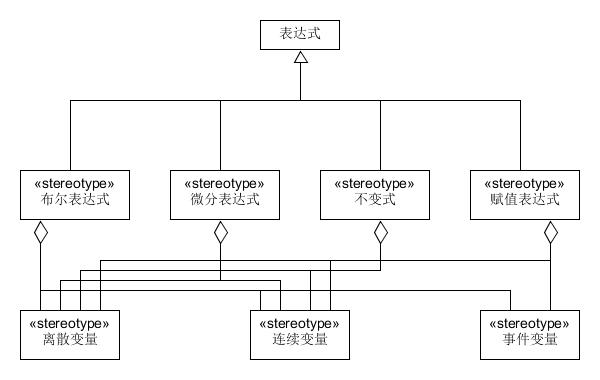
\includegraphics[width=4.8in]{expression.jpg}
	\caption{扩展的MARTE变量和表达式}
	\label{expression}
	\end{figure}
	
	\begin{myDef}布尔表达式\end{myDef}
	布尔表达式(Boolean Expression)由变量和逻辑运算符按一定语法规则组成。从最基本的层次来说,所有的布尔表达式,不论它的长短如何,其值只能是$TRUE$或$FALSE$。布尔表达式中所包含的变量可以是上述的扩展数据类型的任意一种。
	\begin{equation}
	\phi_{bol}::=A(x) \,|\, \phi_{1}\bowtie\phi_{2} \,|\, \neg\phi \,|\, \phi_{1}\vee\phi_{2} \,|\, \phi_{1}\wedge\phi_{2} \,|\, \forall x \cdot \phi(x) \,|\, \exists x \cdot \phi(x)
	\end{equation}

	\begin{itemize}
	\item $A(x)$表示关于变量$x$的任意代数表达式,包括最基本的算术运算符和常用函数。
	\item $\bowtie$为关系运算符,其值可以为$<$、$\leqslant$、$==$、$\geqslant$、$>$,表示对前后两个布尔表达式$\phi_{1}$和$\phi_{2}$的比较
	\item $\neg$、$\vee$、$\wedge$为最常见的逻辑运算操作。
	\item $\forall x  \cdot \phi(x)$和$\exists x  \cdot \phi(x)$分别表示对于任意变量$x$,关于$x$的表达式$\phi(x)$均满足,存在变量变量$x$使得关于$x$的表达式$\phi(x)$满足。
	\end{itemize}
	
	\begin{myDef}微分表达式\end{myDef}
	微分的中心思想是无穷分割,对于CPES中的连续变量,为了表示其随时间流逝的变化规律,本文使用微分表达式(Differential Expression)来描述连续变量的变化规律。
	
	微分表达式可以表示为:
	\begin{equation}
	\phi_{diff}::=F(x,dx/dt)=0
	\end{equation}
	
	它的语义可以解释为:设$m(t)$为一个连续变量,当$m(t)$是微分方程$F(x,dx/dt)=0$的解时,该微分方程被满足,且连续变量在其定义域上连续变化。
	%对于一个微分方程$\Phi(x,dx/dt)=0$,若$x$是上述方程的解,则微分表达式的形式为
	%\begin{equation}
	%\phi_{diff}::=x'=a
	%\end{equation}
	%即$dx/dt=a$,其中$a$是一个实数,表示连续变量$x$在每单位时间的变化量为$a$。
	
	\begin{myDef}不变式\end{myDef}
	不变式(Invariant)表示在系统运行过程中关于某些变量的约束。例如,对于一个电梯系统,不变式$y<800$表示在电梯运行过程中载重量应当始终小于800千克。不变式的形式化定义如下:
	
	\begin{equation}
	\phi_{inv}::=A(x) \,|\, \phi_{1}\bowtie\phi_{2}
	\end{equation}
	
	其中 $A(x)$表示关于变量$x$的任意代数表达式,包括最基本的算术运算符和一些常见的函数;$\bowtie$表示关系运算符,即$<$、$\leqslant$、$\geqslant$、$>$,$=$和$\not=$。

	\begin{myDef}赋值表达式\end{myDef}
	当$x$和$a$对应的数据类型相同时,赋值表达式(Assignment Expression)
	\begin{equation}
	\phi_{assig}::=x:=a
	\end{equation}
	表示将表达式$a$的值赋给变量$x$。在系统建模中,赋值表示变量的更新,即系统中的事件对变量造成的影响。

\section{MARTE/UML模型的扩展}
	UML中的模型可分为静态视图和动态视图,静态视图用于刻画系统的拓扑结构,动态视图用于描述系统的动态行为。静态视图包括类图、构件图、部署图等,动态视图包括用例图、顺序图、活动图、状态图等,使用者可以根据需要选择合适的模型。在继承了UML多视图建模特性的基础上,本文扩展了以下MARTE/UML模型:
	\begin{itemize}
	\item 静态视图:类图
	\item 交互视图:顺序图
	\item 行为视图:状态图
	\end{itemize}
	
	类图通过描述系统中存在的类以及类之间的关系来确定系统元素,类可以实例化为顺序图中的对象;顺序图展示了系统不同部分之间的控制流,包括可能存在的消息同步机制;状态图通过状态和迁移来描述某一对象的内部行为,顺序图中对象的内部活动可以由状态图来建模。
	
	本文在类图、顺序图和状态图中添加了建模CPES所需要的能量、混成和随机信息,给出了其对应的元模型以及语法、语义的定义。
	
%\subsection{UML用例图的扩展}	
	%用例图主要用来描述“用户、需求、系统功能单元”之间的关系。它展示了一个外部用户能够观察到的系统功能模型图。帮助开发团队以一种可视化的方式理解系统的功能需求。用例图实际上并没有描述软件系统的组织结构,而是描述了形成系统体系结构的动力。
		
	%参与者(actor)是在系统之外与系统交互的某人或某事物,它代表对象的某一个方面,并不一定作为一个独立的实体存在。用例(use case)是UML中非常重要的一个概念,在整个模型驱动软件开发过程中,用例处于一个中心地位。它是对一组动作序列的抽象描述,系统执行这些动作序列,产生相应的结果。这些结果要么反馈给参与者,要么作为其他用例的参数。关系(relation)是指用例与用例之间、参与者与用例之间的联系。主题(subject)是由一组用例所描述的一个类,这个类通常是一个系统或者子系统。
	
	%本文假设一个用例对应系统的一个功能,通过用例图直观反映系统被使用的情况以及不同参与者对系统控制。另外,通过OCL语言标注的方式注明每一个用例所相关的能源类型,结合用例被使用的情况,可以定义不同能源对系统的重要性。

	%\begin{figure}[!t]
	%\centering
	%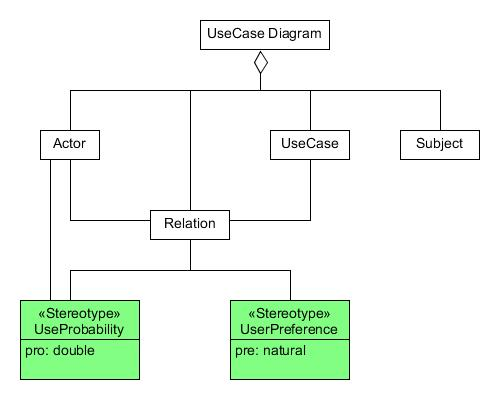
\includegraphics[width=4in]{metamodel-UD.jpg}
	%\caption{扩展的用例图元模型}
	%\label{metamodel-UD}
	%\end{figure}
	
	%ESHMARTE用例图可以用一个五元组来表示:
	
	%\begin{equation}
	%UseCase\ Diagram\ UD=<Actor, Pro, UseCase, Pref, Rel>
	%\end{equation}
	
	%其中,
	%\begin{itemize}
	%\item $Actor$是系统的所有参与者的集合,它对应于一个字符串类型的变量来唯一标识参与者的名称;
	%\item $Pro$是是概率的集合,取值范围为$[0,1]$。用例图中,概率$pro$体现在$actor$和$usecase$上,分别表示系统选择某个用户参与的概率与系统中某个用例被使用的概率。
	%\item $UseCase$代表系统中所有的用例,每个用例都必须有一个区别于其他用例的名称,其值是互不相同的字符串,也对应于一个概率$pro$代表这个用例被系统使用的概率,即$usecase=<ucname,ucpro>$。
	%\item $Pref$是参与者对用例控制的优先级的表示,为整型变量,$pref$值越小则优先级越高。
	%\item 在用例图中,关系$Rel$分为参与者与用例的关系和用例之间的关系两种。参与者和用例的关系可以用$Actor \times Pro \times Pref \rightarrow UseCase$来描述,即参与者与某个用例的关联关系中还增添了参与者使用这个用例的概率与参与者对这个用例使用的优先级。$UseCase \times UseCase \rightarrow String$可以描述用例之间的关系,用例图中涉及的关系有:关联、泛化、包含、扩展,即字符串的取值可以为以上四种之一。
	%\end{itemize}
				
	%由上述扩展的用例图的定义可知,在原有的用例图基础上,增加了随机、控制优先级和能源支持的类型三种信息。
	
	%通过在用例图中添加概率的方式,我们可以得到某个用例在系统中被使用的概率,直观反映该用例的重要程度。关于某个用例在系统中被使用的概率可以通过所有与其相关联的参与者以及参与者使用该用例的概率计算而得。对于某个用例$uc_{k}$,假设参与者$actor_{i}$使用系统的比率为$p_{a_{i}}$,在使用系统的前提下,使用用例$uc_{k}$的概率为$p_{ij}$,则得到用例$uc_{k}$被使用的概率$P_{uc_{k}}= \sum_{i=1}^N(p_{a_{i}}\times p_{ij})$($N$为所有使用用例$uc_{k}$的参与者数量)。当然,如果一个用例被使用的概率是已知的,那么直接对其进行标注即可。
	
	%\begin{figure}[!t]
	%\centering
	%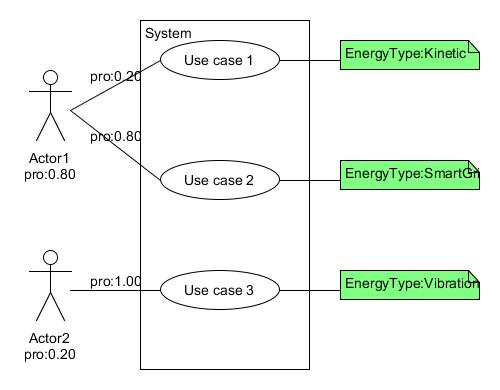
\includegraphics[width=4in]{example-UD.jpg}
	%\caption{ESHMARTE用例图示例}
	%\label{example-UD}
	%\end{figure}	
		
	%在CPES中,控制系统可能为多个参与者所使用,表现在模型中,即有多个参与者与某个用例关联。此时,$pref$的值表示了不同参与者对用例使用的优先级,值越小则优先级越高。同一个用例的所有关联的参与者的$pref$值不同。
	
	%而能源的类型可以通过OCL语言注释的形式添加在用例上。主要的的能源类型有$Vibration Energy$、$Thermal Energy$、$Kinetic Energy$、$Acoustic Energy$和$Biochemical Energy$等。
	
	%通过ESHA用例图新增的建模信息可以帮助分辨在一个多控制系统中,当对某一个控制器的控制发生矛盾时,不同参与者的优先级选择;并直观地体现出了不同用例被使用的概率,侧面反映了用例之间的重要性顺序;以及能源类型备注的方式反映了每种能源对于系统的贡献值和重要性。
\subsection{MARTE/UML类图的扩展}
	类是面向对象系统中最重要的构造块,是对一组具有相同属性、操作、关系和语义的对象的描述。类图可以帮助界定系统中的元素,是系统建模设计的基础。
	
	CPES中存在着大量能耗实体,即系统中那些运作耗能的部件,如空调、照明系统等。同时,系统中又存在一些部件,能够为系统提供能量,如太阳能电池、电网等。因此,在对CPES进行建模时,对这些实体添加合适的信息描述其对系统能量的影响是必要的。此外,一个CPES中,能量的来源可能多种多样,对能量来源进行分类标注可以帮助观测到不同能源对系统的重要性。
	
	在MARTE中,$HW\_Power$包中定义了$HW\_PowerSupply$衍型来描述能量补给,但仅仅将$HW\_Battery$作为唯一补给来源。事实上,能量的补给来源多种多样,包括热能、动能、生物能等等。在这里,对$HW\_PowerSupply$衍型进行如图\ref{harvestor}的扩展,即能量补给来源可分为:电网、太阳能、振动产能、热产能、运动产能、生化能和声波产能。
	
	\begin{figure}[!t]
	\centering
	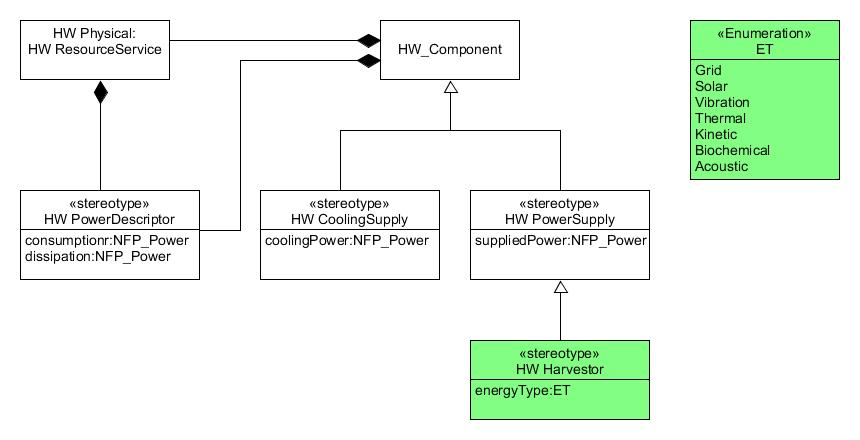
\includegraphics[width=4.2in]{harvestor.jpg}
	\caption{$HW PowerSupply$衍型的扩展}
	\label{harvestor}
	\end{figure}
	
	%在MARTE的GRM包中定义了$ResourceUsage$来描述对于资源的使用,以$energy:NFP\_Energy$的形式来描述某个类造成的能耗。结合此定义,我们将MARTE/UML类图扩展,其元模型如图\ref{metamodel-class}所示,即,对于CPES,系统中包含两类特殊衍型的对象:能量供给对象和耗能对象。
	
	扩展的MARTE/UML类图元模型如图\ref{metamodel-class}所示:1)类的属性中可以包含连续变量,用微分表达式来表示;2)类可以分为两种——耗能类和供能类。MARTE定义的$ResourceUsage$衍型可以定义耗能类,其属性包括耗能功率、工作时间和总能耗。结合上述定义的$HW Havestor$衍型,可以定义供能类,并利用$energyType$标记值来描述能量的来源。
	
	\begin{figure}[!t]
	\centering
	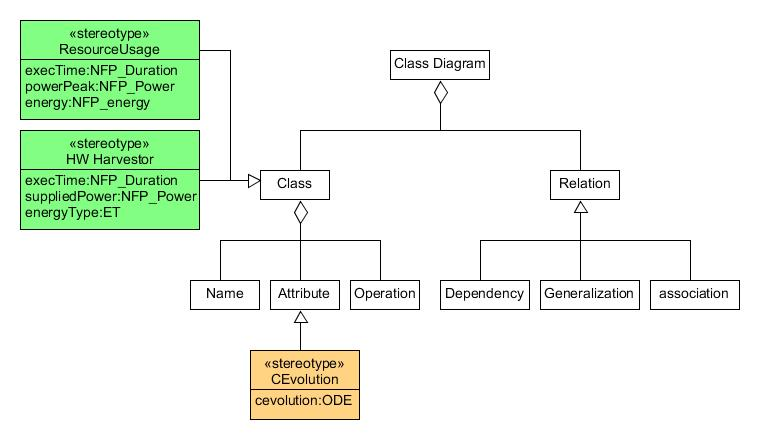
\includegraphics[width=4.8in]{metamodel-CD.jpg}
	\caption{扩展的类图元模型}
	\label{metamodel-class}
	\end{figure}
	
\subsection{MARTE/UML顺序图的扩展}	
\label{2.3.2}
	在一个待开发的系统中,任何对象都不是孤立存在的,系统中的这些对象通过消息进行交互,顺序图(Sequence Diagram)可以对系统中的交互行为进行建模,并以图形化的方式展现。

	顺序图用二维的方式来显示交互:其中,横轴代表参与交互的每个对象,纵轴表示每个对象的生命线(lifeline),即参与交互的时间。对象间的水平箭头代表它们之间消息的传递。当一个对象发送或者接收消息时,即被触活,在模型中用一个瘦高的矩形表示,被称作控制焦点(execution occurrence)。与UML1.x相比,UML2.0顺序图增加了很多可以表达各种分支、循环等情况的组合片段(combined fragments),使得顺序图建模的语义更加丰富。
	
	在CPES中,由于物理环境的开放性,不同对象之间消息的传递可能存在随机性,例如,在某个场景中,用户这个对象有一定的概率将空调度数设置得更高,也有一定概率将度数设置得更低,即在3.2.1节中定义的离散概率选择行为。除此之外,在对象的执行过程中,可能会要求系统满足某些约束,如电梯在上升的过程中要求电梯内的人不超过规定的承载量。	
	
	一个扩展的MARTE/UML顺序图可以用以下六元组表示:
	\begin{equation}
	Sequence\ Diagram\ SD=<Obj, Msg, Exec, Frag, Point, Evn>
	\end{equation}
	
	其中,
	\begin{itemize}
	\item $Obj$是有穷对象的集合,可用字符串标识对象名及其所属类名,例如:$printer:Appliance$。
	\item $Msg$是顺序图中所有消息内容的集合,它由标识符和发送对象、接受对象组成:$msg=(ctn,src,tgt)$。消息标识符$ctn$通常为$operation(parameters)$的形式,如$sendTempData(td)$表示消息内容为传递温度数据,参数为$td$。
	\item $Exec$是控制焦点的集合,表示对象执行一个动作所经历的时间段,对于每一个$exec\in Exec$对应于自己所属的对象$exec.obj\in Obj$。
	\item $Frag$是所有组合片段的集合。顺序图的各基本构成元素,可以通过组合片段封装起来,以表达不同的语义。组合片段包括:循环(loop)、分支(alt、opt)、中断(break)、临界区(critical)、并行(par)和引用(ref)等。一个$frag\in Frag$是一个三元组:$frag=(name,type,area)$,包含组合片段的名称、类型和操作域。
	\item $p \in Point$称为位点,是顺序图中所有对象生命周期上时间点的集合,代表了消息发送和接收的顺序。一个位点$p$是一个四元组:$(exec,frag,rs,order)$,其中$exec$表示位点属于哪一个控制焦点,$frag$代表位点所属的组合片段,$rs$是收发标志位,代表在该位点是接收消息还是发送消息,其取值为$\{0,1\}$,$0$代表接收消息,$1$代表发送消息。顺序图中对象的生命线并不表示精确的时间关系,但同一条生命线上的位点的先后顺序是固定的,$p.order$是位点值,其取值范围是非零自然数,代表该位点在所属对象上按时间先后顺序的排列序号。
	\item 对于每个消息$m\in Msg$,与两个事件相关联:消息的发送事件$!m$和消息的接收事件$?m$。$!m$和$?m$为同步事件。$Evn$为顺序图中所有消息事件的集合。一个消息事件$evn$包含消息内容和消息所处的位点:$evn=(msg,p)$,位点的收发标志位决定该消息事件的类型。即根据消息事件$evn$的位点的标志位$evn.p.rs$的值,可以将消息事件划分为发送消息事件$SE$和接收消息事件$RE$,且$SE \cap RE = \emptyset$。
	\end{itemize}
	
	下面,重点解释顺序图中消息事件执行顺序和组合片段的含义。
	
	\textbf{消息事件执行顺序}:顺序图中对象的生命线并不表示精确的时间,不同对象间的消息事件执行的时间顺序无法比较,但同一个对象生命线上的消息事件存在事件执行的先后顺序,因此,消息事件的执行顺序默认为偏序关系,也就是弱序列。这种弱序列关系的具体含义是:1)消息执行的最终结果是不可改变的;2)同一生命线上的不同消息事件按照先后顺序依次发生;3)不同生命线上的不同消息事件的发生顺序无法确定。
	
	\textbf{组合片段}:在图形中,组合片段表示为一个生命线上的矩形区域,其左上角有一个小五边形,其中的文字被称作标签,表示组合片段的类型。UML2.0顺序图中定义了12种组合片段,下面对常用的几种组合片段作出解释:
	\begin{itemize}
	\item 可选执行:标签为$opt$。用一个方括号括起来的布尔表达式表示进入$opt$组合片段的监护条件,当布尔表达式为真时,执行组合片段内的消息交互内容。
	\item 条件执行:标签为$alt$。组合片段内部用虚线分割成几个区域,每个区域有自己的执行监护条件,这些监护条件的交集为空。若所有监护条件均不满足,则不执行组合片段,否则执行监护条件满足的那一个区域。
	\item 并行执行:标签为$par$。同样使用虚线把组合片段内部划分为几个分区,每个分区表示一个并发执行。当进入组合片段时,同时执行所有分区,但每个分区内部的消息序列是顺序执行的,而不同分区的消息执行则存在交替的关系。这种并行执行的方式在现实生活中很常见。
	\item 循环执行:标签为$loop$。在组合片段内部区域中,设置执行的监护条件,若条件满足,则循环执行$loop$中的序列,不满足则跳出。在标签中还可以设置区间参数来表示循环执行的最少和最多次数。如$loop(1,10)$表示最少执行1次,最多执行10次。
	\end{itemize}
	
	扩展的顺序图元模型如图\ref{metamodel-sequence}所示,下面对MARTE/UML顺序图中扩展部分作出具体阐述。
	
	\begin{figure}[!t]
	\centering
	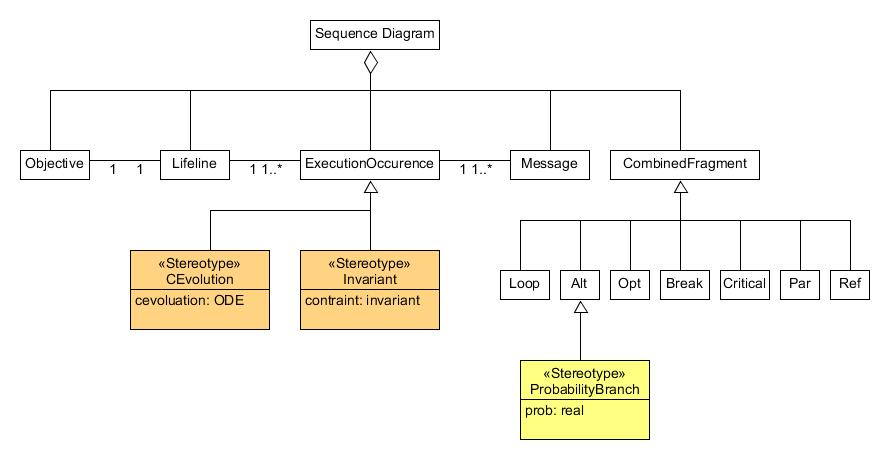
\includegraphics[width=5in]{metamodel-SD.jpg}
	\caption{扩展的顺序图元模型}
	\label{metamodel-sequence}
	\end{figure}
	
	在CPES中,离散概率选择随机行为普遍存在,对$alt$操作符进行扩展可以使其描述这种随机行为——即不同分区的选择不是由监护条件决定,而是由每一分区的执行概率决定。系统执行哪一个分区是不确定的,按照概率随机选择。每一个分区$area_{i}$对应于一个取值为$[0,1]$的$prob_{i}$表示该分区被选择的概率。如图\ref{example-SD}所示,在对象$a$发送消息时,有$80\%$的概率发送正确的消息$sendRight(rData)$,$20\%$的概率发送错误消息$sendWrong(wData)$。
	
	\begin{figure}[!t]
	\centering
	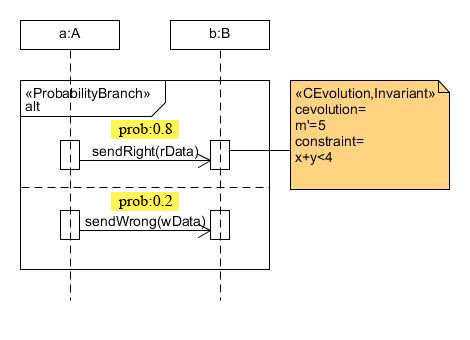
\includegraphics[width=3in]{example-SD.jpg}
	\caption{扩展的顺序图示例}
	\label{example-SD}
	\end{figure}	
	
	CPES是一个混成系统,在某个对象处于执行阶段时,系统可能会存在某些特定的约束,或者某些连续变量的变化率可能维持不变。在对象的控制焦点上,可以通过添加不变式和微分表达式来描述这些信息。如图\ref{example-SD}所示,在对象$b$的第一个控制焦点执行过程中,连续变量$m$的变化率始终为$5$,且变量$x$和$y$之和始终小于4。
	%操作语义的基本思想是用抽象的方法描述语言中每一成分的执行效果,以免所描述的语义依赖于该语言实现时所用的具体计算机,其突出特点在于具有直观的表述方式。
	
	消息事件是顺序图中的重要元素,消息的执行即代表了顺序图的动态逻辑语义。下面结合3.2.2节中定义的事件执行顺序,使用逻辑推导的方式来形式化定义顺序图中\textbf{消息事件执行顺序}的含义:
	\begin{itemize}
	\item $evn_{x}.p.exec.obj==evn_{y}.p.exec.obj \wedge evn_{x}.p.order<(>)evn_{y}.p.order \Longrightarrow evn_{x} \prec(\succ) evn_{y}$
	
	如果消息事件$evn_{x}$和$evn_{y}$的位点同属于一个对象,且$evn_{x}$的位点值小于(大于)$evn_{y}$,则消息事件$evn_{x}$先于(晚于)$evn_{y}$发生。
	\item $evn_{x}.msg==evn_{y}.msg \wedge evn_{x}.p.rs \oplus evn_{y}.p.rs \Longrightarrow evn_{x} \approx evn_{y}$
	
	如果消息事件$evn_{x}$与$evn_{y}$所包含的消息内容相同,且消息对应的位点收发位相异,即一个为消息发送事件,一个为对应的消息接收事件,则$evn_{x}$和$evn_{x}$同时发生。
	\item $\neg (evn_{x}.p.exec.obj==evn_{y}.p.exec.obj) \Longrightarrow evn_{x} \sim evn_{y}$
	
	如果消息事件$evn_{x}$与$evn_{y}$不属于同一个对象,则它们的执行顺序不可判定。
	\end{itemize}
	
	消息事件执行顺序比较的是单个消息事件之间的时间先后顺序。而\textbf{消息事件执行序列}是相对于整个顺序图而言的,它将消息事件按照执行顺序依次排列,并用逗号隔开(本文定义的消息事件是同步事件,执行序列里可以仅列出所有发送事件或所有接收事件),形如:$ES=\{evn_{1},evn_{2},... \}$。

	一个顺序图的消息执行序列是不确定的,原因如下:1)不同生命线上消息的执行顺序不能确定;2)组合片段$opt$、$alt$中消息执行的不同选择让消息事件执行序列的结果具有不确定性,使得顺序图产生语义分歧。下面,针对$opt$和$alt$操作符对消息事件执行序列的影响作出形式化解释:
	
	\begin{itemize}
	\item $evn_{x}.p.frg.type==opt \Longrightarrow  \{ ES_{1},evn_{x},ES_{2} \} | \{ ES_{1},ES_{2} \} $
	
	如果消息事件$evn_{x}$属于一个$opt$组合片段,设$ES_{1}$是$opt$组合片段之前的消息执行序列,$ES_{2}$是$opt$组合片段之后的消息执行序列。由于条件满足时,$opt$操作域内的消息事件才会被执行,所以顺序图的消息执行序列为$\{ ES_{1},evn_{x},ES_{2} \} $或者$\{ ES_{1},ES_{2} \}$。
	\item $evn_{x}.p.frg.type==alt \wedge evn_{y}.p.frg.type==alt \wedge evn_{x}.p.frg.name==evn_{y}.p.frg.name \Longrightarrow \{ ES_{1},evn_{x},ES_{2} \} | \{ ES_{1},evn_{y},ES_{2} \}$
	
	如果消息事件$evn_{x}$和$evn_{y}$同属于一个$alt$组合片段,设$ES_{1}$是$alt$组合片段之前的消息执行序列,$ES_{2}$是$alt$组合片段之后的消息执行序列。由于$alt$选择的互斥性,则顺序图的消息执行序列为$\{ ES_{1},evn_{x},ES_{2} \}$或$\{ ES_{1},evn_{y},ES_{2} \}$。
	\item $evn_{x}.p.frg.type==alt \wedge evn_{y}.p.frg.type==alt \wedge evn_{x}.p.frg.name==evn_{y}.p.frg.name \wedge evn_{x}.p.frg.area.prob==p_{1} \wedge evn_{y}.p.frg.area.prob==p_{2} \Longrightarrow \{ ES_{1},evn_{x},ES_{2} \}_{p_{1}} | \{ ES_{1},evn_{y},ES_{2}\}_{p_{2}} $
	
	如果消息事件$evn_{x}$和$evn_{y}$同属于一个$alt$组合片段设$ES_{1}$是$alt$组合片段之前的消息执行序列,$ES_{2}$是$alt$组合片段之后的消息执行序列。由于$alt$选择的互斥性,则顺序图的消息执行序列有$p_{1}$的可能性为$\{ ES_{1},evn_{x},ES_{2} \}$,$p2$的可能性为$\{ ES_{1},evn_{y},ES_{2} \}$。
	\end{itemize}
	上述推导过程考虑的是单个事件的情形,对于可选片段区域中包含多个事件的情形,所得消息执行序列的结果是类似的。
	
\subsection{MARTE/UML状态图的扩展}
\label{2.3.3}
	顺序图提供了控制流随时间推移的可视化轨迹,但它无法表现单个对象内部的状态变化。而在系统的建模、设计中,这些动态细节的刻画是必需的。因此,需要状态图来对单个对象的生命周期进行描述。
	
	状态图(State Chart)用来表示一个对象在它的生命周期中对外部事件的响应、状态的变化、生命周期的变迁,以及对过去行为的依赖。它将对象与其外部世界分离开来,从局部视角出发,独立考察其行为。
	
	一个扩展的MARTE/UML状态图定义如下:
	\begin{equation}
	State\ Chart\ SC=(State, s_{0}, Inv, Diff, Distr, \tau, Evn, Grd, Prob, Act,Eng)
	\end{equation}
	
	其中,
	\begin{itemize}
	\item $State$为研究对象所有状态的集合。
	\item $s_{0}$为初始状态。
	\item $Inv$代表所有状态上的约束,以不变式的形式描述。
	\item $Diff$是微分表达式的集合,描述了在某个状态下连续变量随时间变化的速率。
	\item $Distr$是时延概率分布,描述了在某个状态下每个时刻发生迁移的概率。
	\item $\tau$是从一个状态到另一个状态的迁移的集合。
	\item $Evn$是所有触发事件的集合,UML中允许没有触发事件的迁移,被称作完成迁移。
	\item $Grd$为所有监护条件的集合,以布尔表达式的形式描述。
	\item $Prob$对应于$[ 0,1 ]$上的实数,代表概率值。
	\item $Act$是迁移发生后带来的效应,通常由赋值表达式组成。
	\item $Eng$表示系统的能耗函数,根据能耗在状态图中产生的位置不同,可以分为:$S \rightarrow R$和$\tau \rightarrow R$两种。能耗值为正代表系统消耗能量,为负代表系统产生能量。
	\end{itemize}
	
	状态和迁移是状态图中最重要的两个元素,下面分别对它们进行更为详细的解释。
	
	\emph{状态}:对于每一个$s \in State$,有$s = (sname,\phi_{inv},\phi_{diff},\phi_{distr}, \phi_{eng})$,其意义是:对于一个系统状态$s$,具有唯一的字符串型状态名$sname$,且在该状态下,系统中的连续变量的变化率满足$\phi_{diff}$。同时,系统变量满足约束$\phi_{inv}$,当$\phi_{inv}$违背且迁移尚未发生时,系统进入终止状态。$\phi_{distr}$为状态的迁移赋予了随机的特性,即系统在状态$s$停留多久取决于时延概率分布$\phi_{distr}$,它定义了系统在每一个时间点发生迁移的概率,即刻画了时延随机行为。$\phi_{eng}$是能量的微分表达式,定义了在状态$s$上能量的变化率。
	
	\emph{迁移}:$\tau:State \times Evn \times Grd \times Prob \times Act \times Eng \rightarrow State$。即迁移是系统由一个源状态$src$向目标状态$tgt$的转变。在触发事件发生的情况下,迁移必须满足一定的监护条件才能发生。$prob\in[0,1]$定义了迁移从源状态到某个目标状态的概率值,对于状态$s$,在相同的触发事件和监护条件下,若其对应于$N$个目标状态,则其到所有目标状态的概率之和为1,即$\sum_{i=1}^N prob_{i} =1$。若在某触发事件和监护条件下,不存在概率分支情况,则迁移是确定的。$Eng:\tau \rightarrow R$定义了迁移$\tau$造成的能耗。
	
	图\ref{metamodel-SC}为扩展状态图的元模型,通过元模型,可以更直观地体现本文所做的扩展:
	\begin{figure}[!t]
	\centering
	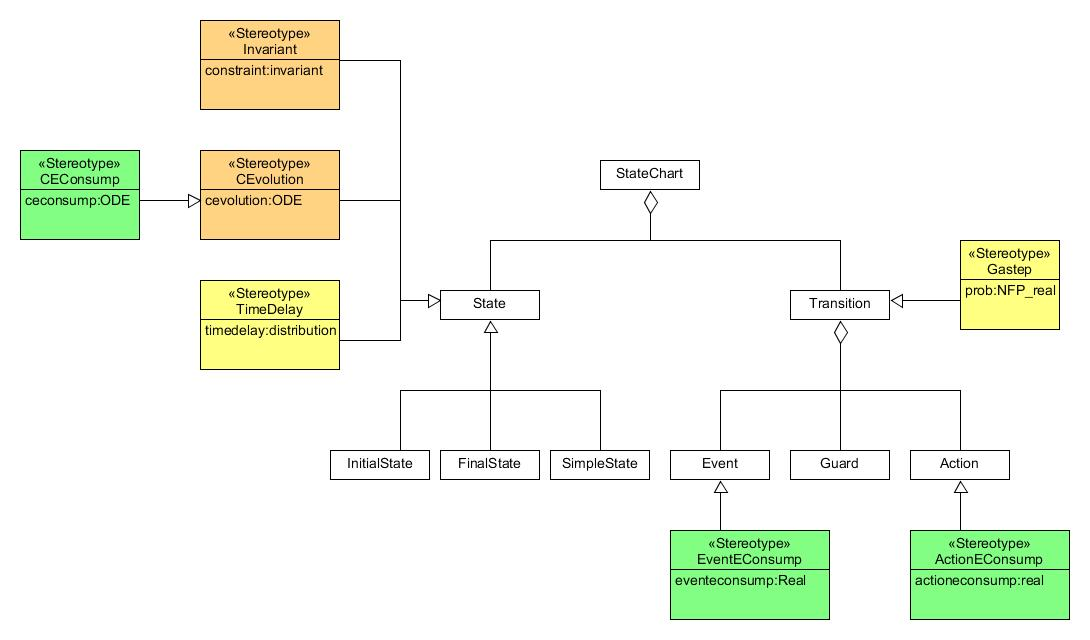
\includegraphics[width=6in]{metamodel-SC.jpg}
	\caption{扩展的状态图元模型}
	\label{metamodel-SC}
	\end{figure}	
	
	\begin{itemize}
	\item 针对CPES的混成特性,对状态增加了$CEvolution$衍型,用微分表达式来刻画系统中连续变量随时间的变化速率;
	\item 针对CPES中存在的两种随机行为,在状态上添加了$TimeDelay$衍型,并使用时延概率分布来描述时延随机行为;而迁移上则利用MARTE原有的$Gastep$衍型刻画了离散概率选择行为;
	\item 在状态图中,根据产生的位置不同可将能耗分为两类:1)在状态上产生的能耗,此时能量是以连续变量的形式通过微分表达式来定义其随时间变化的速率,并结合实际在状态上的停留时间计算而得;2)在迁移上产生的能耗,迁移的触发事件和动作事件的执行可能伴随能量的产生与消耗,与状态上的能量不同,迁移是不耗时的,因此用一个离散的实数值来记录迁移造成的能耗。
	\end{itemize}
	
	图\ref{example-SC}为扩展的MARTE/UML状态图的简单示例,其中,$state1$为$CEvolution$衍型的状态,在该状态下,连续变量$s$随时间的变化率为2,;$state1$在$event$事件的触发下,有$80\%$的可能性迁移至$state2$状态,$20\%$的可能性迁移至$state3$状态,同时,$event$事件会带来两个单位的能耗;在$state2$状态下,系统每单位时间耗能为5,在$state3$状态下,系统每单位时间耗能为10。
	%此处的示例没有列举出所有扩充的信息,在第五章会结合具体案例展现扩展的MARTE/UML的使用。
	
	\begin{figure}[!t]
	\centering
	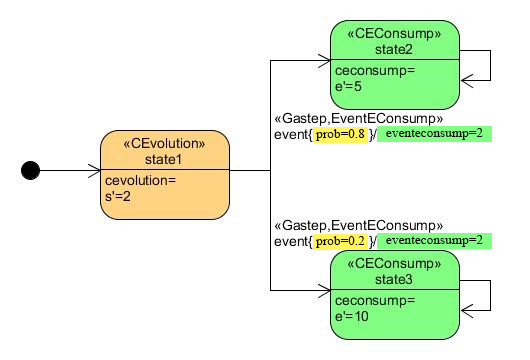
\includegraphics[width=3.5in]{example-SC.jpg}
	\caption{扩展的状态图示例}
	\label{example-SC}
	\end{figure}
	
	同样地,为了准确定义状态图的动态语义,这里使用逻辑推导规则对状态图中的两种迁移作出语义解释。
	
	顺序图中的主要对象是消息事件,其动态逻辑语义可以由消息执行序列表示,而状态图中最重要的元素是状态和迁移,由于本文定义的迁移已经包含了对应的源状态和目标状态的信息,因此,迁移序列$TS=\{ \tau_{1},\tau_{2},...  \}$即可描述状态图由初始状态发生迁移、逐步演化的过程。对于一个状态图而言,由于离散概率选择和状态上时延概率分布的存在,迁移序列是不确定的。
	
	\begin{itemize}
	\item 离散迁移:
	
	$ \tau_{i}.src==\tau_{j}.src \wedge \tau_{i}.evn==\tau_{j}.evn \wedge \tau_{i}.evn==1 \wedge \tau_{i}.grd==\tau_{j}.grd \wedge \phi_{grd_{i}}==TRUE \Longrightarrow \{ TS_{1},\tau_{i}... \}_{\tau_{i}.prob} | \{ TS_{1},\tau_{j}... \}_{\tau_{j}.prob}$ 
	
	设$TS_{1}$为$\tau_{i}$之前的迁移序列,当迁移$\tau_{i}$和$\tau_{j}$所对应的源状态、触发事件和监护条件均相同,且触发事件发生、监护条件满足时,它们被触发的概率由各自的迁移概率值$prob$决定,即系统的迁移序列有$\tau_{i}.prob$的概率为$\{ TS_{1},\tau_{i}... \}$,有$\tau_{j}.prob$的概率为$\{ TS_{1},\tau_{j}... \}$。对于包含多个概率选择的迁移情况,结果类似。
	\item 时延概率迁移:
	
	上述离散迁移仅仅考虑了迁移的概率选择对系统迁移序列的影响,并没有考虑状态上时间延迟的随机性。$\tau_{i\_c_{i}}$表示迁移$\tau_{i}$在其源状态$\tau_{i}.rs$上停留的时间为$c_{i}$。
	设$TS_{1\_C_{1}}$为$\tau_{i}$之前的迁移序列,即系统执行迁移序列$TS_{1}$的耗时为$C_{1}$,则$\{TS_{1\_C_{1}},\tau_{i\_c_{1}}...\}_{\tau_{i}.rs.\phi_{distr}(c_{1})} | ... | \{TS_{1\_C_{1}},\tau_{i\_c_{i}}...\}_{\tau_{i}.rs.\phi_{distr}(c_{i})}$表示对应的时延概率迁移序列。
	\end{itemize}
	
\section{本章小结}
	UML是最常用的系统建模语言之一,MARTE是针对实时嵌入式系统的UML profile,MARTE/UML模型提供了强大的实时性、嵌入式方面的建模能力。但对于智能建筑等CPES的混成、随机和能量感知特性,MARTE/UML建模方式仍然存在一定的局限性。针对此问题,本章首先定义了CPES中的两种随机行为;接着给出了MARTE元素的扩展,包括数据类型和表达式;最后结合MARTE,扩展了UML的类图、顺序图和状态图,给出了其元模型和语法语义,以支持CPES系统的建模。本章给出了扩展模型的简单示例,关于扩展模型的实际应用,可参考第五章案例部分。
	


